\section{Model}
\label{sec:model}
\newcommand{\tex}[1]{20-model/#1}

%\input{\tex{01-summary-of-notation.tex}}

To permit non-preemptive jobs that utilize thread-level schedulers, a
new model is proposed in this work. The set of ${n}$ multi-threaded
tasks is given by ${\tasks}$ ${= \{\task{0}, \task{1}, ...,
\task{n-1}\}}$. Each job of a task ${\task{i} = (\period{i}, \deadline{i}, \taskthreads{i}, c_i:\mathbb{N} \mapsto \mathbb{R}^+)}$ has a minimum
inter-arrival time of \period{i} and relative deadline
\deadline{i}. For every job release of \task{i}, a positive integer
\taskthreads{i} identical threads are released.  Each thread of
\task{i} executes over the same object \object{i} on the shared 
processor. An object is a set of executable machine instructions,
mapping to one set of in memory addresses, such that all threads
execute the same instruction from the same address. All threads share
the same deadline as their job. The worst-case execution time (WCET)
of \task{i} is a function of the number of threads per job,
\wcet{i}{\taskthreads{i}}.

\input{\tex{20-execution-model}}

%\begin{wrapfigure}[7]{i}{.35\linewidth}
\begin{figure}[b]
  \centering
  \begin{subfigure}{.35\linewidth}
    \centering
    \includegraphics[width=\linewidth]{preemptivity}
    \caption{Scheduling Behavior}
    \label{fig:preemptivity}
  \end{subfigure}
  \begin{subfigure}{.58\linewidth}
    \centering
    \includegraphics[width=\linewidth]{process}  
    \caption{Schedulability and Transformable Task Sets}
    \label{fig:process}
  \end{subfigure}
  \caption{Scheduling and Schedulability of the Proposed Model}
\end{figure}
%\end{wrapfigure}



Thread-level scheduling algorithms must be characterized by a WCET
function ${c_i(m_i)}$ for ${m_i}$ threads per job and ${c_i(m_i)}$ must be
strictly increasing discrete and concave (detailed in
Subsection~\ref{sec:discrete-growth}). Thread-level schedulers that
produce concave ${c_i(m_i)}$ functions establish a relationship
between the execution requirements of a task and the number of
threads, where the requirement for one job of ${m_i}$ threads is less
than ${m_i}$ jobs of one thread. For \texttt{BUNDLE}-based schedulers,
concavity is the result of the inter-thread cache benefit, where
${c_i(m) - c_i(m - 1) \ge c_i(m+1) - c_i(m)}$; it is this
relationship the proposed scheduling behavior and analysis seek
to exploit.

Not all tasks and thread-level schedulers will produce concave WCET
functions. For a task \task{i} with a convex WCET function (where
there is no benefit in grouping threads together), the
${m_i}$ threads of \task{i} may be replaced with ${m_i}$
single-threaded tasks. These single-threaded have vacuously concave
WCET functions by virtue of executing no more than one thread.

The task set \tasks{} provided by the system designer to
schedulability analysis is referred to as the task set
\emph{specification}. Commonly~\cite{Baruah:1990,Liu:1973,Baruah:2005,Bertogna:2011,Burns:1995,Buttazzo:2011}, task set specifications are immutable
in hard-real time models. The number of tasks, their
WCET time, period, and deadline are provided by the system
designer, not to be changed. Schedulability analysis determines if
the task set specification is feasible. In this work, task sets are
transformable (obeying some restrictions).

Transformation of a task set exploits the concavity of execution
requirements, redistributing the threads of individual tasks to
multiple tasks. A greater number of threads per job reduces the WCET
of a task but increases the non-preemptive execution
requirement. Conversely, a fewer number of threads per task increases
the total WCET for all tasks while decreasing the non-preemptive
execution requirement. Schedulability analysis in this non-preemptive
setting  encompasses the search for a distribution of the fixed number
threads from the task set specification to a variable number of tasks,
resolving the tension between a greater number of tasks and a
greater number of threads per task to find a feasible task set. 
 
Under the proposed model, schedulability analysis is a process that
begins by considering the current task set named the \emph{anterior}
task set \supts{}. If the set is schedulable, the set is unmodified and
processing ceases with a positive result. If the task set \supts{}
cannot be scheduled as described, the task set is transformed into a
\emph{posterior} task set \tasks{}, and processed again as an anterior
set. Processing ceases with a negative result when there are no
available transformations of \supts{}.

%% \begin{figure}[ht]
%%   \centering
%%   \includegraphics[width=.58\linewidth]{process}  
%%   \caption{Schedulability and Transformable Task Sets}
%%   \label{fig:process}
%% \end{figure}


Figure~\ref{fig:process} illustrates the schedulability analysis
process. Division is the transformative operation of the process and
is described in Subsection~\ref{sec:dividing}. The figure highlights the
ability of a single task set to be both anterior and posterior to
different sets during processing. To aid in explanation, properties of a
task may be referred to in terms of the set the task was transformed
from and to. By example, if the number of threads assigned to \task{i}
in the anterior set \supts{} is reduced by one in the posterior task
set \tasks{}, the posterior threads of \task{i} may be written as
${m_i = \hat{m}_i - 1}$.

As a process, schedulability analysis of the specified task set serves
two purposes under this model. The first, is to determine if there exists a
posterior task set which is feasible. Second, to produce the feasible
posterior task set if one exists. It is the feasible posterior task
set \tasks{} found by schedulability analysis that is then
deployed on the target architecture. From the system designer's
perspective, each task ${\task{i} \in \tasks{}}$ of the specified
task set is a request to execute ${m_i}$ threads of the object ${o_i}$
with shared periods ${p_i}$ and deadlines ${d_i}$ for \textbf{any}
posterior task set \tasks{}. A task set specification is flexible,
for one object there may be multiple tasks with variable numbers of
threads per job. However, the specified ${m_i}$ of a task is a ceiling
on any ${m_i}$ of a posterior task. 

\subsection{Dividing and Task Parts}
\label{sec:dividing}

A task set may be transformed by \emph{dividing} tasks of the set.
Dividing a task reduces the number of threads executed by each
job, splitting the anterior task into two or more tasks in the
posterior set. 

\begin{definition}[Task Division]
\label{def:restrict-division}
In the anterior task set \supts{}, a task
${\task{i} = (\period{i}, \deadline{i}, \wcet{i}{\taskthreads{i}})}$
may be \emph{divided} into two (or more) posterior tasks \task{j} and
\task{k} with three restrictions: 1.) the periods of \task{j} and
\task{k} are equal to the period of \task{i} 2.) the relative
deadlines of \task{j} and \task{k} are equal to the deadline of
\task{i} 3.) the sum of threads of \task{j} and \task{k} are equal to
\task{i} 4.) the objects of \task{i}, \task{j}, and \task{k} are
equal. Enumerated, the restrictions are: 

\begin{tabular}{m{5cm} m{5cm}}
  \begin{enumerate}
    \item{\period{i} = \period{j} = \period{k}}
    \item{\deadline{i} = \deadline{j} = \period{k}}
  \end{enumerate} &
  \begin{enumerate}
    \setcounter{enumi}{2}
    \item{\taskthreads{i} = \taskthreads{j} + \taskthreads{k}}
    \item{\object{i} = \object{j} = \object{k}}
  \end{enumerate}
\end{tabular}
\end{definition}

\begin{definition}[Partial Tasks]
\label{def:partial-tasks}
When an anterior task \task{i} is divided into \task{j} and \task{k}
posterior tasks, \task{j} and \task{k} are referred to as
\emph{partial tasks} or \emph{parts} of \task{i}.
\end{definition}

\begin{definition}[Partial Task Set]
  \label{def:partial-task-set}
  For convenience, the set of posterior tasks of \task{i} is denoted
  \Partial{i} and called the \emph{partial task set} of \task{i}, 
  where ${m_i = \sum_{\task{k} \in \Partial{i}} m_k}$.
\end{definition}
\input{\tex{10-growth}}

%
% XXX-CT: Transitive and reflexive definitions
%  These were removed, they may need to be included in the future.
%
% BEGIN COMMENT
%% The parts relationship is transitive: if \task{j} is a part of
%% \task{i}, and \task{j} is divided into parts \task{o} and \task{p},
%% then \task{o} and \task{p} are parts of both \task{j} and
%% \task{i}. The relationship is also reflexive: \task{i} is a part of
%% \task{i}.
% END COMMENT
%

